\subsection{Collars}
\begin{enumerate}
\item A \defn{collar} consists of LP @ \(K\) + SC @ \(K'\) with \(K'>K\) (both
options are on the same asset and have the same expiration date):
\begin{center}
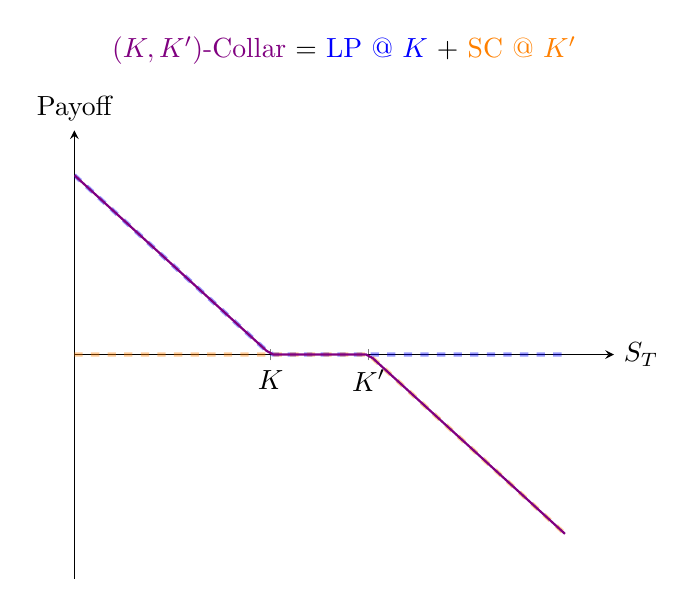
\begin{tikzpicture}[
declare function={
lc(\x) = (\x <= 3) * 0 + (\x > 3) * (\x - 3);
lp(\x) = (\x <= 2) * (2 - \x) + (\x > 2) * 0;
sp(\x) = (\x <= 2) * -(2 - \x) + (\x > 2) * 0;
sc(\x) = (\x <= 3) * 0 + (\x > 3) * -(\x - 3);
}
]
\begin{axis}[domain=0:5, ymin=-2.5, ymax=2.5, xmax=5.5, axis y line=left, axis x line=middle,
title={{\color{violet}\((K, K')\)-Collar} = {\color{blue}LP @ \(K\)} + {\color{orange}SC @ \(K'\)}},
title style={yshift=0.5cm}, xtick={2,3}, xticklabels={\(K\), \(K'\)},
ytick=\empty,
ylabel={Payoff},
ylabel style={at={(axis description cs:0,1)}, anchor=south, rotate=-90},
xlabel={\(S_T\)},
xlabel style={anchor=west}, samples=75
]
\addplot[blue, dashed, ultra thick, opacity=0.4] {lp(x)};
\addplot[orange, dashed, ultra thick, opacity=0.4] {sc(x)};
\addplot[violet, thick] {lp(x)+sc(x)};
\end{axis}
\end{tikzpicture}
\end{center}

\item The main usage of collar is to insure a long position in
\faIcon{apple-alt}.  Recall that a \emph{floor} is a way to hedge such risk (by
adding LP on top of long \faIcon{apple-alt}). The ``initial positive'' part of
payoff (P/L) of LP helps reducing the risk:

\begin{center}
\begin{tikzpicture}[
declare function={
lp(\x) = (\x <= 2) * (1.5-\x) + (\x > 2) * (-0.5);
la(\x) = (\x-2.2);
}
]
\begin{axis}[domain=0:5, ymin=-2.5, ymax=2.5, xmax=5.5, axis y line=left, axis x line=middle,
title={{\color{violet}Floor} = {\color{blue}Long \faIcon{apple-alt}} + {\color{orange}LP @ \(K\)}},
xtick={2}, xticklabel={\(K\)}, xticklabel style={yshift=0.7cm, xshift=0.2cm},
ytick={-2.2},
yticklabel={\(-S_0e^{rT}\)},
ylabel={P/L},
ylabel style={at={(axis description cs:0,1)}, anchor=south, rotate=-90},
xlabel={\(S_T\)},
xlabel style={anchor=west}, samples=75
]
\addplot[blue, thick, dashed, opacity=0.5]{la(x)};
\addplot[orange, thick, dashed, opacity=0.5]{lp(x)};
\addplot[violet, thick]{la(x)+lp(x)};
\draw[opacity=0.4, ForestGreen, line width=0.2cm, line cap=round, line join=round] (0,-0.7) -- (2,-0.7) -- (2.6,-0.1);
\node[ForestGreen] at (1.2,-0.4) {hedged \faIcon{shield-alt} risk};
\end{axis}
\end{tikzpicture}
\end{center}


\item However, for the floor, we need to pay the put option price \(P_0(K)\).
To reduce the initial expense, a \emph{collar} can be used instead of LP.
(Note that the payoff graph of collar also has an ``initial positive'' part.)

\begin{note}
We call ``long \faIcon{apple-alt} + collar'' as \defn{collared
\faIcon{apple-alt}}.  (We usually use this terminology for \emph{stock}:
collared stock.)
\end{note}

Since the time-0 value of a collar is \(P_0(K)-C_0(K')\), which is less than
\(P_0(K)\), this insurance is ``cheaper''. Of course there is no ``free lunch''
and the thing we give up is the profit ``potential'':
\begin{center}
\begin{tikzpicture}[
declare function={
lp(\x) = (\x <= 2) * (1.5-x) + (\x > 2) * -0.5;
sc(\x) = (\x <= 3) * 0.3 + (\x > 3) * -(x-3.3);
la(\x) = (\x-2.2);
}
]
\begin{axis}[
domain=0:5, ymin=-2.5, ymax=2.5, xmax=5.5, axis y line=left, axis x line=middle,
title={{\color{violet}Collared \faIcon{apple-alt}} = {\color{blue}Long \faIcon{apple-alt}} + {\color{orange}\((K, K')\)-Collar}},
title style={yshift=0.5cm},
xtick={2,3}, xticklabels={\(K\),\(K'\)}, xticklabel style={yshift=0.7cm, xshift=0.2cm},
ytick={-2.2},
yticklabel={\(-S_0e^{rT}\)},
ylabel={P/L},
ylabel style={at={(axis description cs:0,1)}, anchor=south, rotate=-90},
xlabel={\(S_T\)},
xlabel style={anchor=west}, samples=75,
legend entries={Collared \faIcon{apple-alt}, Floor},
legend style={legend pos=outer north east}
]
\addplot[violet, thick]{la(x) + lp(x) + sc(x)};
\addplot[opacity=0.4, magenta, thick]{la(x)+lp(x)};
\addplot[blue, thick, dashed, opacity=0.5]{la(x)};
\addplot[orange, thick, dashed, opacity=0.5]{lp(x) + sc(x)};
\draw[opacity=0.4, ForestGreen, line width=0.2cm, line cap=round, line join=round] (0,-0.4) -- (2,-0.4) -- (2.3,-0.1);
\end{axis}
\end{tikzpicture}
\end{center}
After taking a collar, the range of P/L gets restricted to a ``narrow''
range, just like a physical \emph{collar} put around the neck of an animal that
restricts its ``movement''. By varying \(K\) and \(K'\) (such that \(K'>K\) of
course), we can ``place'' the restriction at different ``locations'' and
control its ``strength'' (how ``narrow'').

\item The time-0 value of a collar \(P_0(K)-C_0(K')\) can be positive,
negative, or zero (depending on the choice of \(K\) and \(K'\)). If it is zero,
the collar is called \defn{zero-cost collar}.

\begin{intuition}
For zero-cost collar, the ``protection'' sources completely from the profit
potential given up, since we do not pay any money for this insurance.
\end{intuition}

\item However, if the strike price \(K\) specified is ``too high'', then it is
impossible to construct a zero-cost collar, as suggested by the following
result:
\begin{proposition}
\label{prp:k-high-no-zero-cost-collar}
If \(K\ge S_0e^{rT}\) (the no-arbitrage forward price), then for any \(K'>K\),
\[
C_0(K')<P_0(K)
\]
(so the time-0 value of the collar is always positive).
\end{proposition}
\begin{pf}
For any \(K'>K\),
\begin{align*}
P_0(K)&=C_0(K)+Ke^{-rT}-S_0&\text{(put-call parity)}\\
&>C_0(K')+{\color{violet}K}e^{-rT}-S_0&\text{(\cref{prp:call-put-price-strike-relationship})}\\
&\ge C_0(K')+{\color{violet}S_0e^{rT}}e^{-rT}-S_0\\
&=C_0(K').
\end{align*}
\end{pf}
\end{enumerate}
\subsection{Straddles}
\label{subsect:straddles}
\begin{enumerate}
\item Sometimes speculators are \emph{neither bullish nor bearish}, and
they speculate the \emph{volatility} instead. They are not speculating the
\emph{direction} of future price movement, but its \emph{magnitude} (large
movement \faIcon{arrow-right} high ``volatility''; small movement
\faIcon{arrow-right} low ``volatility'').
\item Some option strategies for volatility speculation are discussed in
\cref{subsect:straddles,subsect:strangles,subsect:butterfly-sprd}.
\item A \defn{straddle} is a combination of call and put on the same asset
\faIcon{apple-alt}, with the same strike price and expiration date.

\item The payoff graph of straddle:
\begin{center}
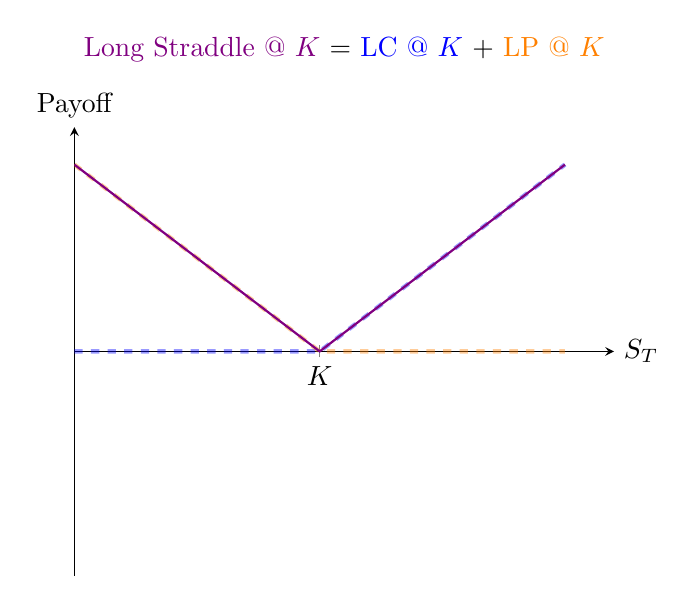
\begin{tikzpicture}[
declare function={
lc(\x) = (\x <= 2.5) * 0 + (\x > 2.5) * (\x - 2.5);
lp(\x) = (\x <= 2.5) * (2.5 - \x) + (\x > 2.5) * 0;
}
]
\begin{axis}[domain=0:5, ymin=-3, ymax=3, xmax=5.5, axis y line=left, axis x line=middle,
title={{\color{violet}Long Straddle @ \(K\)} = {\color{blue}LC @ \(K\)} + {\color{orange}LP @ \(K\)}},
title style={yshift=0.5cm}, xtick={2.5}, xticklabels={\(K\)},
ytick=\empty,
ylabel={Payoff},
ylabel style={at={(axis description cs:0,1)}, anchor=south, rotate=-90},
xlabel={\(S_T\)},
xlabel style={anchor=west}, samples=75
]
\addplot[blue, dashed, ultra thick, opacity=0.4] {lc(x)};
\addplot[orange, dashed, ultra thick, opacity=0.4] {lp(x)};
\addplot[violet, thick] {lc(x)+lp(x)};
\end{axis}
\end{tikzpicture}
\end{center}
\begin{note}
The ``shape'' of the graph looks like the act of ``straddling'' (sitting
astride), from ``top view''.
\end{note}


\item The time-0 price of a straddle is \(C_0+P_0\), which is positive. Hence,
its P/L graph can be obtained by shifting its payoff graph downward:
\begin{center}
\begin{tikzpicture}[
declare function={
lc(\x) = (\x <= 2.5) * 0 + (\x > 2.5) * (\x - 2.5);
lp(\x) = (\x <= 2.5) * (2.5 - \x) + (\x > 2.5) * 0;
}
]
\begin{axis}[domain=0:5, ymin=-3, ymax=3, xmax=5.5, axis y line=left, axis x line=middle,
title={{\color{violet}Long Straddle}},
title style={yshift=0.5cm}, xtick={2.5}, xticklabels={\(K\)},
ytick={-0.8}, yticklabels={\(-(C_0+P_0)e^{rT}\)},
ylabel={P/L},
ylabel style={at={(axis description cs:0,1)}, anchor=south, rotate=-90},
xlabel={\(S_T\)},
xlabel style={anchor=west}, samples=75
]
\addplot[violet, opacity=0.4, thick] {lc(x)+lp(x)};
\addplot[violet, thick] {lc(x)+lp(x)-0.8};
\draw[-Latex, brown] (1,1.3) -- (1,0.8);
\draw[-Latex, brown] (1.5,0.8) -- (1.5,0.3);
\draw[-Latex, brown] (3.5,0.8) -- (3.5,0.3);
\draw[-Latex, brown] (4,1.3) -- (4,0.8);
\end{axis}
\end{tikzpicture}
\end{center}

\item To speculate \emph{high} volatility (large future price movement in
either direction), one can long straddle.

\item On the other hand, if one want to speculate \emph{low} volatility (small
future price movement in either direction), one can \emph{short} straddle (SC @
\(K\) + SP @ \(K\)).

\item The payoff and P/L graphs of short straddle:
\begin{center}
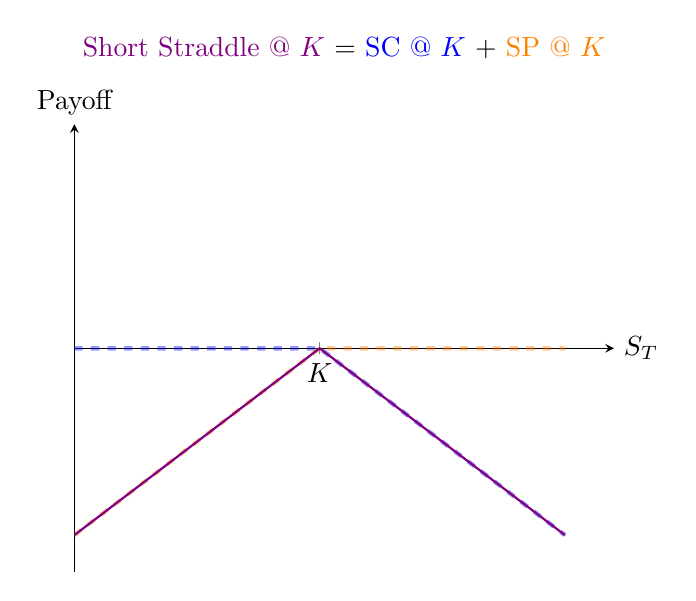
\begin{tikzpicture}[
declare function={
lc(\x) = (\x <= 2.5) * 0 + (\x > 2.5) * (\x - 2.5);
lp(\x) = (\x <= 2.5) * (2.5 - \x) + (\x > 2.5) * 0;
}
]
\begin{axis}[domain=0:5, ymin=-3, ymax=3, xmax=5.5, axis y line=left, axis x line=middle,
title={{\color{violet}Short Straddle @ \(K\)} = {\color{blue}SC @ \(K\)} + {\color{orange}SP @ \(K\)}},
title style={yshift=0.5cm}, xtick={2.5}, xticklabels={\(K\)},
ytick=\empty,
ylabel={Payoff},
ylabel style={at={(axis description cs:0,1)}, anchor=south, rotate=-90},
xlabel={\(S_T\)},
xlabel style={anchor=west}, samples=75
]
\addplot[blue, dashed, ultra thick, opacity=0.4] {-lc(x)};
\addplot[orange, dashed, ultra thick, opacity=0.4] {-lp(x)};
\addplot[violet, thick] {-lc(x)-lp(x)};
\end{axis}
\end{tikzpicture}

\begin{tikzpicture}[
declare function={
lc(\x) = (\x <= 2.5) * 0 + (\x > 2.5) * (\x - 2.5);
lp(\x) = (\x <= 2.5) * (2.5 - \x) + (\x > 2.5) * 0;
}
]
\begin{axis}[domain=0:5, ymin=-3, ymax=3, xmax=5.5, axis y line=left, axis x line=middle,
title={{\color{violet}Short Straddle}},
title style={yshift=0.5cm}, xtick={2.5}, xticklabels={\(K\)},
ytick={0.8}, yticklabels={\((C_0+P_0)e^{rT}\)},
ylabel={P/L},
ylabel style={at={(axis description cs:0,1)}, anchor=south, rotate=-90},
xlabel={\(S_T\)},
xlabel style={anchor=west}, samples=75
]
\addplot[violet, opacity=0.4, thick] {-lc(x)-lp(x)};
\addplot[violet, thick] {-lc(x)-lp(x)+0.8};
\draw[-Latex, brown] (1,-1.3) -- (1,-0.8);
\draw[-Latex, brown] (1.5,-0.8) -- (1.5,-0.3);
\draw[-Latex, brown] (3.5,-0.8) -- (3.5,-0.3);
\draw[-Latex, brown] (4,-1.3) -- (4,-0.8);
\draw[opacity=0.5, red, line width=0.2cm, line cap=round] (1,-0.7) -- (0,-1.7);
\draw[opacity=0.5, red, line width=0.2cm, line cap=round] (4,-0.7) -- (5,-1.7);
\node[red] () at (4.5,-0.3) {high risk \faIcon{exclamation-triangle}!};
\end{axis}
\end{tikzpicture}
\end{center}
\begin{warning}
A short straddle is highly risky and has \emph{unlimited} potential loss. This
strategy caused the collapse of \emph{Barings Bank}!
\end{warning}
\end{enumerate}
\subsection{Strangles}
\label{subsect:strangles}
\begin{enumerate}
\item A \emph{strangle} is another strategy for speculating volatility which is
``cheaper'' than straddle. To achieve a lower cost, call (put) option with
higher (lower) strike price is used, through which some profit potential is
given up.

\item A \((K-\Delta,K+\Delta)\)-\defn{strangle} is a combination of call and
put with strike prices \(K+\Delta\) and \(K-\Delta\) respectively, on the same
asset \faIcon{apple-alt}, with the same expiration date.

\begin{note}
The time-0 price of the \((K-\Delta,K+\Delta)\)-strangle is
\(C_0(K+\Delta)+P_0(K-\Delta)\), which is lower than the price of the straddle
@ \(K\): \(C_0(K)+P_0(K)\) since \(C_0(K+\Delta)<C_0(K)\) and
\(P_0(K-\Delta)>P_0(K)\) by \cref{prp:call-put-price-strike-relationship}.
\end{note}
\item The payoff and P/L graphs of long strangle:
\begin{center}
\begin{tikzpicture}[
declare function={
lc(\x) = (\x <= 3) * 0 + (\x > 3) * (\x - 3);
lp(\x) = (\x <= 2) * (2 - \x) + (\x > 2) * 0;
}
]
\begin{axis}[domain=0:5, ymin=-3, ymax=3, xmax=5.5, axis y line=left, axis x line=middle,
title={{\color{violet}Long \((K-\Delta,K+\Delta)\)-Strangle} = {\color{blue}LC @ \(K+\Delta\)} + {\color{orange}LP @ \(K-\Delta\)}},
title style={yshift=0.5cm}, xtick={2,3}, xticklabels={\(K-\Delta\),\(K+\Delta\)},
ytick=\empty,
ylabel={Payoff},
ylabel style={at={(axis description cs:0,1)}, anchor=south, rotate=-90},
xlabel={\(S_T\)},
xlabel style={anchor=west}, samples=75
]
\addplot[blue, dashed, ultra thick, opacity=0.4] {lc(x)};
\addplot[orange, dashed, ultra thick, opacity=0.4] {lp(x)};
\addplot[violet, thick] {lc(x)+lp(x)};
\end{axis}
\end{tikzpicture}

\begin{tikzpicture}[
declare function={
lc(\x) = (\x <= 3) * 0 + (\x > 3) * (\x - 3);
lp(\x) = (\x <= 2) * (2 - \x) + (\x > 2) * 0;
}
]
\begin{axis}[domain=0:5, ymin=-3, ymax=3, xmax=5.5, axis y line=left, axis x line=middle,
title={{\color{violet}Long Strangle}},
title style={yshift=0.5cm}, xtick={2,3}, xticklabels={\(K-\Delta\),\(K+\Delta\)},
xticklabel style={yshift=0.7cm},
ytick=\empty,
ylabel={P/L},
ylabel style={at={(axis description cs:0,1)}, anchor=south, rotate=-90},
xlabel={\(S_T\)},
xlabel style={anchor=west}, samples=75
]
\addplot[violet, thick, opacity=0.4] {lc(x)+lp(x)};
\addplot[violet, thick] {lc(x)+lp(x)-0.5};
\draw[->, brown] (1,0.95) -- (1,0.6);
\draw[->, brown] (1.5,0.45) -- (1.5,0.1);
\draw[->, brown] (3.5,0.45) -- (3.5,0.1);
\draw[->, brown] (4,0.95) -- (4,0.6);
\end{axis}
\end{tikzpicture}
\end{center}

\item The payoff and P/L graphs of short strangle:
\begin{center}
\begin{tikzpicture}[
declare function={
lc(\x) = (\x <= 3) * 0 + (\x > 3) * (\x - 3);
lp(\x) = (\x <= 2) * (2 - \x) + (\x > 2) * 0;
}
]
\begin{axis}[domain=0:5, ymin=-3, ymax=3, xmax=5.5, axis y line=left, axis x line=middle,
title={{\color{violet}Short \((K-\Delta,K+\Delta)\)-Strangle} = {\color{blue}SC @ \(K+\Delta\)} + {\color{orange}SP @ \(K-\Delta\)}},
title style={yshift=0.5cm}, xtick={2,3}, xticklabels={\(K-\Delta\),\(K+\Delta\)},
xticklabel style={yshift=0.7cm},
ytick=\empty,
ylabel={Payoff},
ylabel style={at={(axis description cs:0,1)}, anchor=south, rotate=-90},
xlabel={\(S_T\)},
xlabel style={anchor=west}, samples=75
]
\addplot[blue, dashed, ultra thick, opacity=0.4] {-lc(x)};
\addplot[orange, dashed, ultra thick, opacity=0.4] {-lp(x)};
\addplot[violet, thick] {-lc(x)-lp(x)};
\end{axis}
\end{tikzpicture}

\begin{tikzpicture}[
declare function={
lc(\x) = (\x <= 3) * 0 + (\x > 3) * (\x - 3);
lp(\x) = (\x <= 2) * (2 - \x) + (\x > 2) * 0;
}
]
\begin{axis}[domain=0:5, ymin=-3, ymax=3, xmax=5.5, axis y line=left, axis x line=middle,
title={{\color{violet}Short Strangle}},
title style={yshift=0.5cm}, xtick={2,3}, xticklabels={\(K-\Delta\),\(K+\Delta\)},
ytick=\empty,
ylabel={P/L},
ylabel style={at={(axis description cs:0,1)}, anchor=south, rotate=-90},
xlabel={\(S_T\)},
xlabel style={anchor=west}, samples=75
]
\addplot[violet, thick, opacity=0.4] {-lc(x)-lp(x)};
\addplot[violet, thick] {-lc(x)-lp(x)+0.5};
\draw[->, brown] (1,-0.95) -- (1,-0.6);
\draw[->, brown] (1.5,-0.45) -- (1.5,-0.1);
\draw[->, brown] (3.5,-0.45) -- (3.5,-0.1);
\draw[->, brown] (4,-0.95) -- (4,-0.6);
\end{axis}
\end{tikzpicture}
\end{center}

\item A comparison of P/L graphs of long strangle and long straddle:
\begin{center}
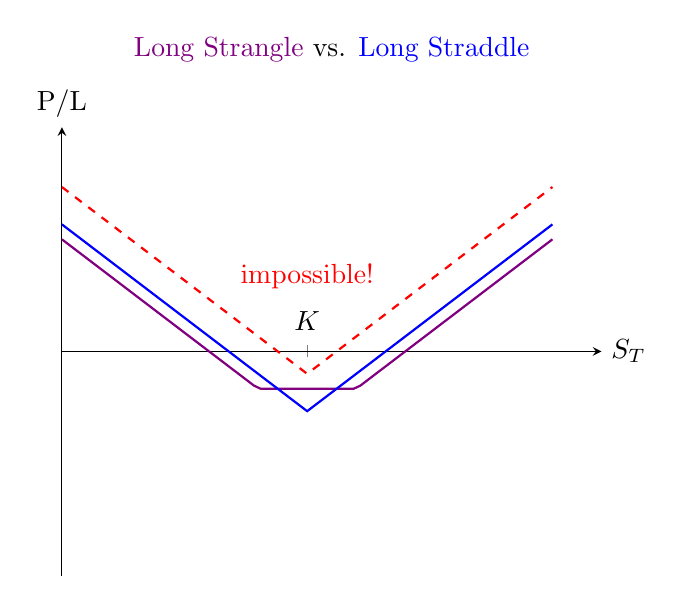
\begin{tikzpicture}[
declare function={
lc3(\x) = (\x <= 3) * 0 + (\x > 3) * (\x - 3);
lp2(\x) = (\x <= 2) * (2 - \x) + (\x > 2) * 0;
lc(\x) = (\x <= 2.5) * 0 + (\x > 2.5) * (\x - 2.5);
lp(\x) = (\x <= 2.5) * (2.5 - \x) + (\x > 2.5) * 0;
}
]
\begin{axis}[domain=0:5, ymin=-3, ymax=3, xmax=5.5, axis y line=left, axis x line=middle,
title={{\color{violet}Long Strangle} vs. {\color{blue}Long Straddle}},
title style={yshift=0.5cm}, xtick={2.5}, xticklabels={\(K\)},
xticklabel style={yshift=0.7cm},
ytick=\empty,
ylabel={P/L},
ylabel style={at={(axis description cs:0,1)}, anchor=south, rotate=-90},
xlabel={\(S_T\)},
xlabel style={anchor=west}, samples=75
]
\addplot[violet, thick] {lc3(x)+lp2(x)-0.5};
\addplot[blue, thick] {lc(x)+lp(x)-0.8};
\addplot[red, thick, dashed] {lc(x)+lp(x)-0.3};
\node[red] () at (2.5,1) {impossible!};
\end{axis}
\end{tikzpicture}
\end{center}
\begin{note}
Under the no-arbitrage principle, the graphs must cross each other. Otherwise,
arbitrage would be possible.
\end{note}
\end{enumerate}
\subsection{Butterfly Spreads}
\label{subsect:butterfly-sprd}
\begin{enumerate}
\item Recall that short straddle is highly risky. This suggests a need to
\emph{insure} the short straddle, and \emph{butterfly spread} is a strategy
that does this.

\item Recall: P/L graph of short straddle:
\begin{center}
\begin{tikzpicture}[
declare function={
lc(\x) = (\x <= 2.5) * 0 + (\x > 2.5) * (\x - 2.5);
lp(\x) = (\x <= 2.5) * (2.5 - \x) + (\x > 2.5) * 0;
}
]
\begin{axis}[domain=0:5, ymin=-3, ymax=3, xmax=5.5, axis y line=left, axis x line=middle,
title={{\color{violet}Short Straddle}},
title style={yshift=0.5cm}, xtick={2.5}, xticklabels={\(K\)},
ytick={0.8}, yticklabels={\((C_0+P_0)e^{rT}\)},
ylabel={P/L},
ylabel style={at={(axis description cs:0,1)}, anchor=south, rotate=-90},
xlabel={\(S_T\)},
xlabel style={anchor=west}, samples=75
]
\addplot[violet, thick] {-lc(x)-lp(x)+0.8};
\draw[opacity=0.5, red, line width=0.2cm, line cap=round] (1,-0.7) -- (0,-1.7);
\draw[opacity=0.5, red, line width=0.2cm, line cap=round] (4,-0.7) -- (5,-1.7);
\node[red] () at (4.5,-0.3) {high risk \faIcon{exclamation-triangle}!};
\end{axis}
\end{tikzpicture}
\end{center}
To insure the short straddle, we need \emph{both} ``initial positive'' and
``later positive'' parts for P/L, so \emph{long strangle} is a good candidate.

\begin{note}
Long straddle is another choice but it would just close out the short
straddle position (if they are both @ \(K\)), which is not very interesting.
\end{note}

\item A \((K-\Delta,K+\Delta)\)-\defn{butterfly spread} consists of ``short
straddle @ \(K\)'' + ``long \((K-\Delta,K+\Delta)\)-strangle''.

\item The payoff and P/L graphs of butterfly spread:
\begin{center}
\begin{tikzpicture}[ declare function={
lc3(\x) = (\x <= 3) * 0 + (\x > 3) * (\x - 3);
lp2(\x) = (\x <= 2) * (2 - \x) + (\x > 2) * 0;
lc(\x) = (\x <= 2.5) * 0 + (\x > 2.5) * (\x - 2.5);
lp(\x) = (\x <= 2.5) * (2.5 - \x) + (\x > 2.5) * 0;
}
]
\begin{axis}[domain=0:5, ymin=-3, ymax=3, xmax=5.5, axis y line=left, axis x line=middle,
title={{\color{violet}\((K-\Delta,K+\Delta)\)-Butterfly Spread} 
= {\color{blue}Short Straddle @ \(K\)} + {\color{orange}Long \((K-\Delta,K+\Delta)\)-Strangle)}},
title style={yshift=0.5cm}, xtick={2,3}, xticklabels={\(K-\Delta\),\(K+\Delta\)}, xticklabel style={above=0.2cm},
ytick=\empty,
ylabel={Payoff},
ylabel style={at={(axis description cs:0,1)}, anchor=south, rotate=-90},
xlabel={\(S_T\)},
xlabel style={anchor=west}, samples=75
]
\addplot[violet, thick] {lc3(x)+lp2(x)-lc(x)-lp(x)};
\addplot[orange, dashed, thick, opacity=0.4] {lc3(x)+lp2(x)};
\addplot[blue, dashed, thick, opacity=0.4] {-lc(x)-lp(x)};
\end{axis}
\end{tikzpicture}

\begin{tikzpicture}[
declare function={
lc3(\x) = (\x <= 3) * 0 + (\x > 3) * (\x - 3);
lp2(\x) = (\x <= 2) * (2 - \x) + (\x > 2) * 0;
lc(\x) = (\x <= 2.5) * 0 + (\x > 2.5) * (\x - 2.5);
lp(\x) = (\x <= 2.5) * (2.5 - \x) + (\x > 2.5) * 0;
}
]
\begin{axis}[domain=0:5, ymin=-3, ymax=3, xmax=5.5, axis y line=left, axis x line=middle,
title={{\color{violet}\((K-\Delta,K+\Delta)\)-Butterfly Spread}},
title style={yshift=0.5cm}, xtick={2,3}, xticklabels={\(K-\Delta\),\(K+\Delta\)},
xticklabel style={yshift=0.7cm},
ytick=\empty, ylabel={P/L},
ylabel style={at={(axis description cs:0,1)}, anchor=south, rotate=-90},
xlabel={\(S_T\)},
xlabel style={anchor=west}, samples=75,
]
\addplot[violet, thick] {lc3(x)+lp2(x)-lc(x)-lp(x) + 0.3};
\addplot[violet, thick, opacity=0.4] {lc3(x)+lp2(x)-lc(x)-lp(x)};
\draw[->, brown] (1,-0.45) -- (1,-0.2);
\draw[->, brown] (1.5,-0.45) -- (1.5,-0.2);
\draw[->, brown] (3.5,-0.45) -- (3.5,-0.2);
\draw[->, brown] (4,-0.45) -- (4,-0.2);
\end{axis}
\end{tikzpicture}
\end{center}
\begin{remark}
\item Either of payoff and P/L graphs looks like a ``butterfly'' flying away
(or towards you).
\item The P/L graph is obtained by shifting the payoff graph \emph{upward}
since P/L cannot be always nonpositive (alternatively, the strangle is cheaper
than the straddle \faIcon{arrow-right} time-0 value of butterfly spread is
negative).
\end{remark}
\item A comparison of P/L graphs of butterfly spread and short straddle:
\begin{center}
\begin{tikzpicture}[ declare function={
lc3(\x) = (\x <= 3) * 0 + (\x > 3) * (\x - 3);
lp2(\x) = (\x <= 2) * (2 - \x) + (\x > 2) * 0;
lc(\x) = (\x <= 2.5) * 0 + (\x > 2.5) * (\x - 2.5);
lp(\x) = (\x <= 2.5) * (2.5 - \x) + (\x > 2.5) * 0;
}
]
\begin{axis}[domain=0:5, ymin=-3, ymax=3, xmax=5.5, axis y line=left, axis x line=middle,
title={{\color{violet}\((K-\Delta,K+\Delta)\)-Butterfly Spread} 
= {\color{blue}Short Straddle @ \(K\)} + {\color{orange}Long \((K-\Delta,K+\Delta)\)-Strangle)}},
title style={yshift=0.5cm}, xtick={2,3}, xticklabels={\(K-\Delta\),\(K+\Delta\)}, xticklabel style={above=0.2cm},
ytick=\empty,
ylabel={Payoff},
ylabel style={at={(axis description cs:0,1)}, anchor=south, rotate=-90},
xlabel={\(S_T\)},
xlabel style={anchor=west}, samples=75
]
\addplot[violet, thick] {lc3(x)+lp2(x)-lc(x)-lp(x)};
\addplot[orange, dashed, thick, opacity=0.4] {lc3(x)+lp2(x)};
\addplot[blue, dashed, thick, opacity=0.4] {-lc(x)-lp(x)};
\end{axis}
\end{tikzpicture}

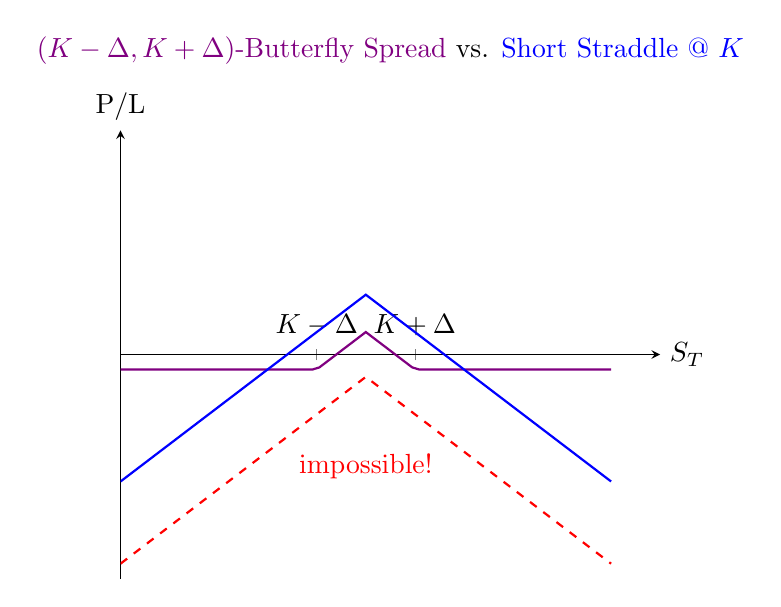
\begin{tikzpicture}[
declare function={
lc3(\x) = (\x <= 3) * 0 + (\x > 3) * (\x - 3);
lp2(\x) = (\x <= 2) * (2 - \x) + (\x > 2) * 0;
lc(\x) = (\x <= 2.5) * 0 + (\x > 2.5) * (\x - 2.5);
lp(\x) = (\x <= 2.5) * (2.5 - \x) + (\x > 2.5) * 0;
}
]
\begin{axis}[domain=0:5, ymin=-3, ymax=3, xmax=5.5, axis y line=left, axis x line=middle,
title={{\color{violet}\((K-\Delta,K+\Delta)\)-Butterfly Spread} vs. {\color{blue}Short Straddle @ \(K\)}},
title style={yshift=0.5cm}, xtick={2,3}, xticklabels={\(K-\Delta\),\(K+\Delta\)},
xticklabel style={yshift=0.7cm},
ytick=\empty, ylabel={P/L},
ylabel style={at={(axis description cs:0,1)}, anchor=south, rotate=-90},
xlabel={\(S_T\)},
xlabel style={anchor=west}, samples=75,
]
\addplot[violet, thick] {lc3(x)+lp2(x)-lc(x)-lp(x) + 0.3};
\addplot[blue, thick] {-lc(x)-lp(x)+0.8};
\addplot[red, dashed, thick] {-lc(x)-lp(x)-0.3};
\node[red] () at (2.5,-1.5) {impossible!};
\end{axis}
\end{tikzpicture}
\end{center}
\begin{note}
Again, under the no-arbitrage principle, the graphs must cross each other
(i.e., the short straddle graph cannot be ``below'' the ``butterfly''!).
\end{note}
\end{enumerate}

